%!TEX program = xelatex
% Note: this template must be compiled with XeLaTeX rather than PDFLaTeX
% due to the custom fonts used. The line above should ensure this happens
% automatically, but if it doesn't, your LaTeX editor should have a simple toggle
% to switch to using XeLaTeX.

\documentclass[
  aspectratio=169, % Uncomment to use an aspect ratio of 16:9 (160 mm by 90 mm)
  %aspectratio=43, % Uncomment to use an aspect ratio of 4:3 (128mm by 96mm)
  t, % Top align all slide content by default
  onlytextwidth, % Typeset content in columns at text width
  10pt, % Default font size, use 10pt for the 16:9 aspect ratio and 8pt for the 4:3 aspect ratio
]{beamer}

\usepackage{../../ImperialTheme/beamer/beamerthemeImperial} % Use the Imperial theme

\def\imagefolder{../../ImperialTheme/beamer/Images}
\def\Rey{\text{Re}}
\title{jeff update} % Presentation title to appear on the title slide and left footers

\subtitle{} % Presentation subtitle to appear on the title slide

\author{Víctor Ballester} % Author name(s) to appear on the title slide

\date{\today} % Presentation date to appear on the title slide and right footers

\begin{document}

\begingroup
\setbeamercolor{background canvas}{bg=ICLLightGrey} % Slide background color
\setbeamercolor{title page title}{fg=ICLBlue} % Title text color
\setbeamercolor{title page subtitle}{fg=ICLBlue} % Subtitle text color
\setbeamercolor{author}{fg=ICLBlue} % Author(s) text color
\setbeamercolor{date}{fg=ICLBlue} % Date text color
\setbeamertemplate{title page}[logo]{\imagefolder/ICL_Logo_Blue.pdf} % Imperial logo color, use 'ICL_Logo_White.pdf' for white and 'ICL_Logo_Blue.pdf' for blue
\frame[plain, s]{\titlepage} % Output the title page with no footer ('plain') and vertically distributed text ('s')
\endgroup

\begin{frame}
	\frametitle{$\Delta n$-factors}
		\begin{columns}[T] % [T] ensures correct vertical alignment
		\begin{column}{0.49\linewidth} % left column
				Difference in computation.
				\begin{itemize}
					\item Jeff (??): First computes the n-factor $n(x)$ curve for the flat plate as a function of $x$. Then, observes the transition location  $x_t^{flat}$ and $x_t^{gap}$ and sets $n_{flat} := n(x_t^{flat})$ and $n_{gap} := n(x_t^{gap})$. Of course since $x_t^{gap} < x_t^{flat}$, then $n_{gap} < n_{flat}$ because $n$ is monotonic.
					\item Victor: Use the definion of $n(x)$ as $\log (A(x)/A_0)$ for both the flat plate and the gap case in different computations. So $n_{flat} = \log (A_{flat}(x_t^{flat})/A_0)$ and $n_{gap} = \log (A_{gap}(x_t^{gap})/A_0)$. Since $A_{gap}(x) > A_{flat}(x)$ then $n_{gap} > n_{flat}$.
				\end{itemize}
				Same physics? idk
		\end{column}
		\begin{column}{0.49\linewidth} % left column
			\begin{figure}[ht]
				\centering
				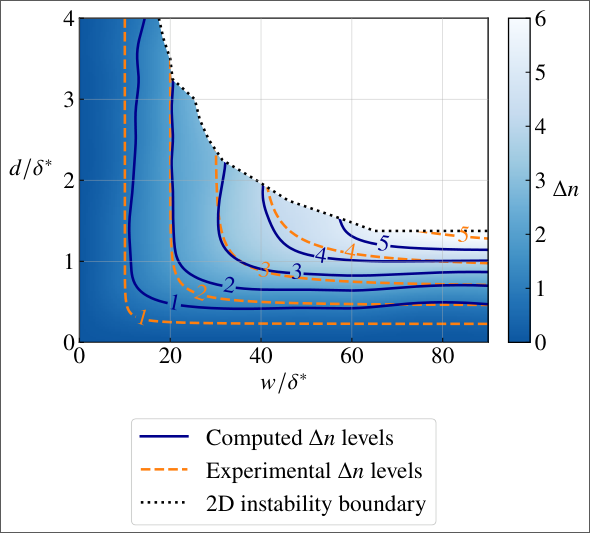
\includegraphics[width=\linewidth]{Images/DeltaN.png}
			\end{figure}
		\end{column}
	\end{columns}
\end{frame}
\begin{frame}
	\frametitle{3d stuff}
  
	\begin{columns}[T] % [T] ensures correct vertical alignment
		\begin{column}{0.49\linewidth} % left column
			\begin{itemize}
				\item Between the 2d and 3d bifurcations, it doesn't seem to be transition, because the streaks in the BL are very week. But of course the integration of time is finite and the velocity evolution inside the gap is not clear (quite chaotic). Could it be that the transition come after a very long time?
			\end{itemize}
			\vspace{-0.5cm}
			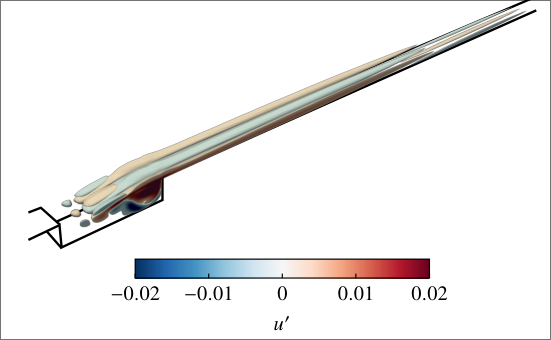
\includegraphics[width=\linewidth]{Images/3dmode.png}
		\end{column}
		\begin{column}{0.49\linewidth} % left column
			\begin{figure}[ht]
				\centering
				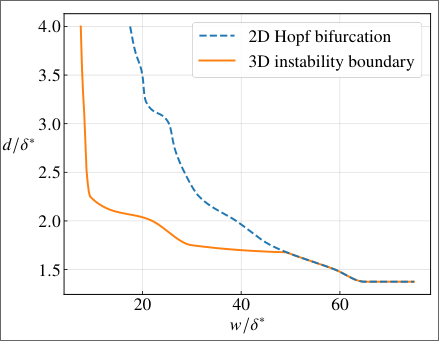
\includegraphics[width=\linewidth]{Images/3d2dbif.png}
			\end{figure}
		\end{column}
	\end{columns}
\end{frame}
\begin{frame}
	\frametitle{Ma number}
  
	\begin{columns}[T] % [T] ensures correct vertical alignment
		\begin{column}{0.49\linewidth} % left column
			\begin{itemize}
				\item Ma number generally destabilizes the system. 
				\item Hoewver Ma = 0.8 seems to behave slightly different thant 0.6 and 0.4. Why???
				\item We also ran incompressible 2d simulations at Re = 2000 (instead of 1000) and the Hopf bifurcation shifts to smaller widths.
			\end{itemize}
		\end{column}
		\begin{column}{0.49\linewidth} % left column
			\begin{figure}[ht]
				\centering
				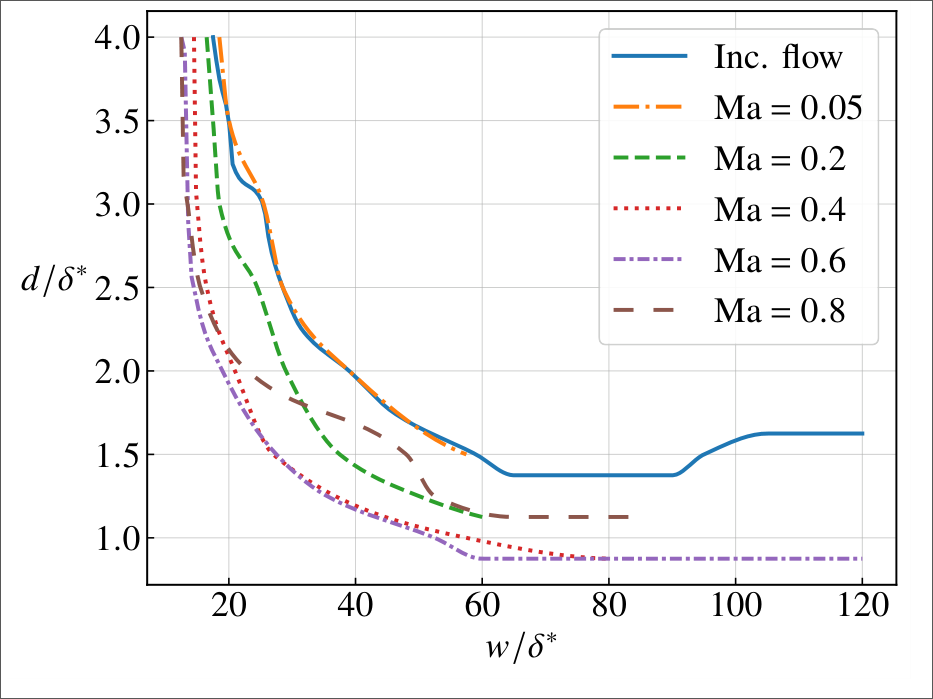
\includegraphics[width=\linewidth]{Images/mabif.png}
			\end{figure}
		\end{column}
	\end{columns}
\end{frame}
\end{document}
